% !TeX root = ../thuthesis-example.tex

\chapter{引言}

\section{问题描述}

行人位置估计是计算机视觉中的经典问题,也是长期以来难以解决的问题。和人脸检测问题相比,由于人体的姿态复杂,变形更大,附着物和遮挡等问题
更严重,因此准确的检测处于各种场景下的行人具有很大的难度。位置估计要解决的问题是:找出图像或视频帧中所有的行人,并估计出每个行人的3D真
实位置。实际上,从要解决的问题上来看,行人位置估计相当于跨摄像头目标跟踪和多目标跟踪的融合,从所需技术上看,其包含行人检测、相机投影、数
据融合、行人重识别等多个领域。


\section{课题研究背景及意义}

近年来,社会科技水平迅速发展,机器学习与人工智能领域在实际社会生活中也得到了越来越广泛的应用。2017年国务院发布的《新一代人工智能发展规划》
中指出:人工智能将成为国与国之间新的竞争领域,人工智能是能够引领未来,颠覆未来的国家战略性技术,我国需要将人工智能技术作为提高国家竞争力,
保障国家安全的重大战略。同时,由于社会信息化水平的迅猛发展,我国近年来监控摄像头在各个公共场所得到迅速普及。在学校、医院、车站、银行甚至是每
个人的家中,监控摄像头的身影无处不在,各种摄像头产生了海量的视频数据,因此,如何利用这些视频数据便成为一个具有相当广阔前景的研究方向。例如,
如今新型冠状病毒肆虐全球,如何利用无处不在的摄像头判断出行人体温,并对其位置加以追踪?又如当今自动驾驶技术飞速发展,如何利用汽车前置摄像头
判断出行人位置,从而确定规避策略?这种背景凸显了计算机视觉技术的关键性。而在计算机视觉领域,机器学习与人工智能技术的广泛应用取得了相当好的
效果。在深度学习方法下,以往在目标跟踪、轨迹检测、视频分类、行为分析、动作识别、自动驾驶等领域棘手的课题也取得了突破性的发展。行人位置估计作为
计算机视觉领域一个关键并具有挑战性的问题也不例外。同时,由于视频序列并非互相独立,而是以时间维度的连续序列,因此在时间的维度上存在动作的连
续性,若对此特点加以挖掘,可大大提升深度学习方法在视频序列分析上的效果。尤其是在多摄像头行人位置估计领域,深度学习方法仍然又很大的探
索空间和应用价值。因此,多摄像头行人位置估计正在受到越来越多的关注和重视。目前,多摄像头行人估计是很多热门技术的基础,在智能监
控、客流量统计和自动驾驶方面均有应用。
	
在智能监控和轨迹预测领域,多视角行人位置估计可获得行人和车辆的行为轨迹,也可以对其未来轨迹进行预测,从而判断那些人物与车辆有意外的危
险,提前发出警告或做好记录,也可以根据行人或车辆的预测轨迹进行警示,以阻止违反交通规则的行为。

在自动驾驶领域,多视角行人位置估计可利用汽车前置摄像头以及周边环境监控摄像头预测交通事故的发生可能性,从而帮助汽车智能选择行进决
策、安排行驶路线、协调速度和方向。

在一般场景下,目前已经存在较高精度的多视角行人位置估计算法。但在较为密集的场景下,目前的算法鲁棒性一般,这是因为较为密集的场景下存
在着比较严重的互相遮挡问题,从而造成对行人特征提取不全、信息缺时的问题。同时,不同摄像头视角的信息也没有得到充分的利用。可见,应对密集场
景下的行人位置估计,提高算法鲁棒性具有着重要的研究意义。



\section{研究背景与现状}

多摄像头行人位置估计问题具有相当多的技术难点,例如行人外观差异大、密集行人的互相遮挡、背景复杂难以分
割、多视角数据融合和行人的重识别、模型复杂检测速度底下等。早期行人位置估计多使用图像处理以及模式识别中的传统方法,准确率较低,效果欠佳。
然而随着深度学习的迅速发展,行人检测和重识别在性能上有了巨大的突破。一方面,越来越多的数据集被发布,例如WildTrack\cite{wildtrack}数据集,
提供了大量的训练样本,促进了深度学习在此领域的应用;另一方面,用于不同研究目的的不同结构的深度学习网络也相继涌现,网络的深度也大幅深入,
大大提高了网络的学习能力和预测精度。下文将对近年来推动多摄像头行人位置估计算法的技术进行介绍。

\subsection{单目行人检测算法}

单目行人检测的任务是通过单个摄像头采集的数据,找出视频帧中的行人,也可显示其位置。检测结果一般用图像中的矩形框来表示。单目行人检测可分
为基于运动检测的算法和基于机器学习的算法。

基于运动检测的算法基本原理是先对视频做背景建模,再利用获取到的背景参考与当前图像序列的当前帧做差分,从而计算出背景图像像素差异,
设定阈值将运动目标和背景进行分割。基于运动检测的经典算法包括单高斯算法、帧间差算法、高斯混合模型分离算法\cite{zivkovic2006efficient}、
VIBE算法\cite{barnich2010vibe}、CodeBook算法\cite{codebook}等,这些传统方法各有特点和优势,但主要流程都是先通过背景建模提取得到视频中的运动目标,再通过分类器来判断出行人。其主要优势在于算法简单、运行比较高效,甚至可以达到实时监测的效果。但这些方法也存在一些缺陷,例如需要摄像头固定,且很容易受到环境和背景噪声的影响,这对环境和设备有很大的要求,并且产生了很多不确定因素。另外,这些方法的一大缺点是只能检测运动目标而不能检测静止目标,这大大增加了算法的局限性。

基于机器学习的算法,基本原理是基于HOG的特征提取和SVM分类器的行人检测。HOG(Histogram of Oriented Gradient)\cite{histograms}特征是
基于本地像素块进行特征直方图提取的一种算法。而SVM(Support Vector Machine)的原理则是通过找到一个超平面使得超平面离最近的样本点距离最大化,以对样本进行分类。然而,HOG和SVM相结合的方法有一个比较大的缺陷就是计算量较大,计算速度比较慢,此外,其对遮挡的鲁棒性很差。此后,积分通道特征(integral channel features)\cite{dollar2009integral}和部分检测的方法也被提出,以对上述方法进行优化。

近年来,由于深度学习方法的迅速发展和应用,单目行人检测算法也迎来了新的研究热潮。MonoPair\cite{monopair}使用经过训练的网络来获取检测到的人或其他目标的3D检测框(bouding box),然后添加成对的空间关系(基于与目标之间中点相关的预测约束),以改进对行人位置估计的结果。MonoLoco\cite{monoloco}在单目行人检测领域提出基于不确定性估计来推断每个行人的2D检测框的深度。它采用2D估计来建模模糊的3D位置,而这种模糊特征与被跟踪人群的内在特征有关。Hayakawa和Dariush\cite{hayakawa}通过引入不对称损失函数改进了MonoLoco的3D位置估计方法。它可以更好地处理了远处行人估计关节的像素相关误差,从而提高了位置估计精度。

\subsection{行人重识别算法}

行人重识别(Person Re-identification, Re-ID)的目标是利用计算机视觉技术在已有的可能来源与非重叠摄像机视域的视频序列中识别出目标行人。在监控视频中,由于相机分辨率和拍摄角度等各种外在条件的限制,往往难以得到目标人物较为清晰的脸部图像,因此人脸识别失效。这种情景就是行人重识别就成为一个重要应用场景。当前行人重识别的研究主要分为两大类:closed-world和open-world。closed-world主要是从行人的检测框图片中去检索目标行人,而open-world重在直接从视频中去检索目标行人,或者是偏向无监督、弱监督学习。目前,机器学习方法在行人重识别算法中得到了广泛应用,其主要包括基于表征学习的Re-ID方法、基于度量学习的Re-ID方法、基于局部特征的Re-ID方法和基于视频序列的Re-ID方法。

表征学习(Representation learning)方法在行人重识别领域的应用很常见。得益于卷积神经网络(Convolutional neural network,CNN)的迅速发展,从图像中根据人物需求提取表征特征的技术越来越成熟。基于特征表示的方法重点在于在光照和视角变化的情况下提高行人图像特征表示模型的鲁棒性。其提取的特征主要有底层视觉特征、中层语义特征和高级视觉特征三个方面。对于底层视觉特征,这种方法主要将图像划分为多个区域,对每个区域底层视觉特征提取后进行组合。由于多数情况下行人衣着颜色比较简单,因此最常用的是RGB、HSV颜色直方图,这是因为颜色特征在不同光照或角度等行人识别的不适环境中具有一定的不变性。此外,还有Haar-like Represention、局部二值模式(LBP)、Gabor滤波器、共生矩阵(Co-occurrence Matrics)等方法提取底层视觉特征。对于中层语义特征,主要是利用行人的颜色、衣服、鞋子、头发长短和是否携带物品等语义信息。将这些语义信息加权与底层视觉信息结合,使得效果有所提升。对于高级视觉特征,主要的特征提取包括视频帧与帧之间的时序信息、图像光流特征、步态或移动轨迹等,如今已经提出了各种各样的方法。例如,Gou\cite{gou2016person}等人提出DynFV(Dynamic Fisher Vector)特征和捕获步态和移动轨迹的Fisher向量编码的密集短轨迹时间金字塔特征,而McLaughlin\cite{mclaughlin2016recurrent}等对图像提取颜色和光流特征,采用卷积神经网络处理得到高层表征,然后用循环神经网络(Recurrent Neural Network, RNN)捕捉时间信息,然后池化得到序列特征。

度量学习(Metric Learning)广泛应用于图像检索领域,因此在行人重识别中也得到了很多应用。度量学习根据同一行人的不同图片相似度大于不同行人的不同图片的原理,设计损失函数,使得相同行人图片的距离更小,而不同行人图片的距离更大。常用的损失函数包括对比损失(Contrastive Loss)、三元组损失(Triplet Loss)、 四元组损失(Quadruplet Loss)、难样本采样三元组损失(triplet hard loss with batch hard mining, TriHard Loss)。不论是上述何种损失,其目标都是保证网络不仅能够在特征空间把正负样本推开,也能保证正样本对之间的距离更近。

局部特征是指对图像中的某一个区域进行特征提取,最后将多个局部特征融合起来作为最终特征。基于局部特征的Re-ID方法主要源于全局特征方法的瓶颈。常用的局部特征提取方法主要有图像切块、利用骨架关键点定位和姿态矫正等。图像切块一般是指将人物boundinb box图像垂直切割为若干份(如图~\ref{fig:part}所示\cite{varior2016siamese}),分别输入网络进行训练。此外,由于图像不对齐,图像切片就会失效,一些论文提出先利用预训练的人体姿态和骨架模型的先验知识,估计出行人关键点后利用仿射变换将关键点对齐,或者直接利用这些关键点来抠出感兴趣区域(Region of Interest, ROI)\cite{zhao2017spindle},最终得到融合全局特征和局部特征的行人重识别特征,从而提高效果。

\begin{figure}
  \centering
  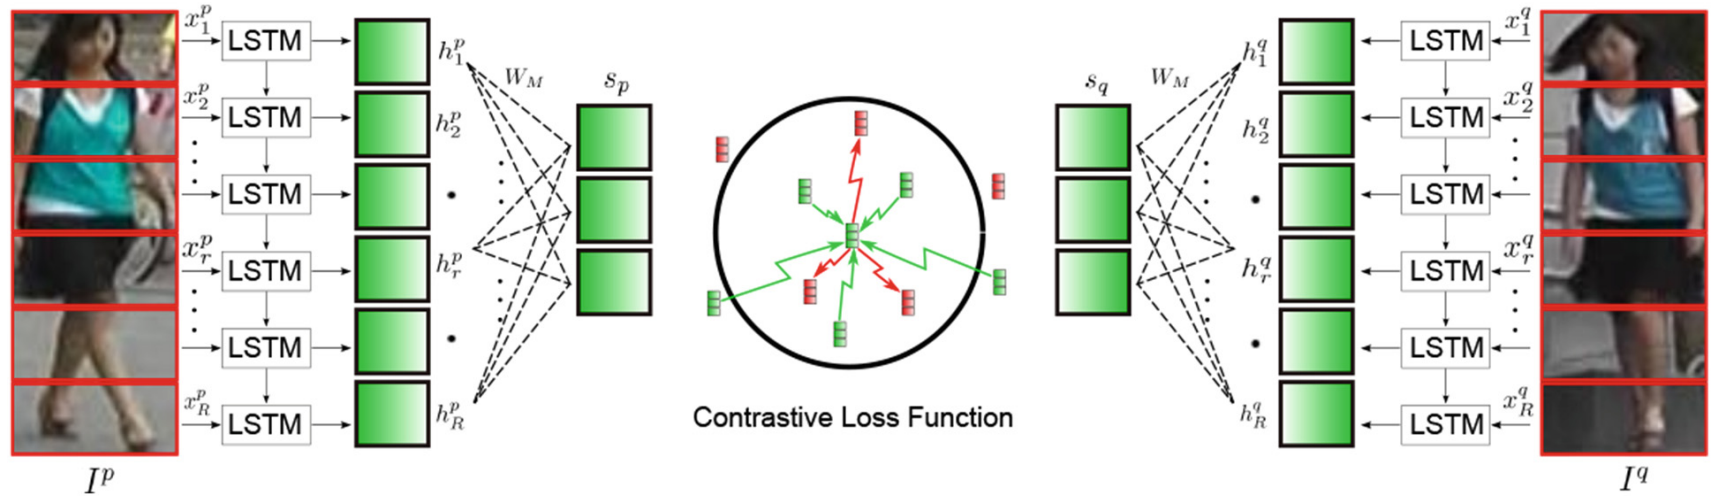
\includegraphics[width=1\linewidth]{切片.png}
  \caption{图片垂直切割后输入LSTM(Long Short-Term Memory)网络后进行特征提取}
  \label{fig:part}
\end{figure}

基于视频序列的Re-ID方法最主要特点是这类方法不仅考虑了图像的内容信息,还考虑了帧与帧之间的运动信息、时序信息等。这类方法主要基于利用CNN提取空间特征的同时,也要利用循环神经网络提取时序特征。 累计运动背景网络(Accumulative Motion Context Network, AMOC)\cite{liu2017video}是代表方法之一,其核心思想在于网络除了要提取序列图像的特征,还要提取运动光流的运动特征,最后再输入RNN来提取时序特征。于是,通过AMOC网络,每个图像序列都能被提取出一个融合了内容信息、运动信息的特征。



\subsection{多摄像头行人位置估计算法}

与单目行人检测算法相比,多摄像头行人位置估计通常来看具有更好的效果,因为多个视角很适合解决复杂遮挡问题\cite{baque2017deep}。

概率占据图方法(Probabilistic Occupancy Map method, POM)\cite{fleuret2007multicamera}通过从多个视角中发掘其中的几何约束,从而得到行人在地面的位置概率的生成模型。POM是在平均场推断常常被自然地用于处理遮挡问题的背景下产生的。同时,为了利用视频的时序信息,概率占据图方法常常与凸最大成本流优化(Convex Max-cost Flow Optimization)\cite{berclaz2009multiple}相结合,应用于行人跟踪的问题中。

在行人比较拥挤的场景中,Ge\cite{ge2010crowd}等人提出采用随机人群配置的随机生成过程建模,然后使用最大后验概率估计来寻找图像观测值的最佳拟合。而Chavdarova\cite{chavdarova2017deep}等人则提出了DeepMCD(Deep Multi-camera Detection)算法,这种方法集成了CNN得到的特征图,并展示了CNN分类器的准确性和可信度可以随着摄像头视角的的增加而提高。为了缓解数据需求问题并提高泛化能力,作者首先使用较大的单目数据集——Caltech数据集\cite{dollar2009pedestrian}来训练得到基础处理网络。之后,CNN被用来使用从基础处理网络中得到的权重数据,并通过并行(Multi-view Stream)的方法处理得到最终的估计结果。作为这种方法的优化,Chavdarova等人后续又在\cite{chavdarova2017deep}中提出了两种多视角数据负挖掘的架构,来更好地训练这种网络。

目前,有一些多视角技术考虑对目标场景进行额外的训练步骤,以更好地利用应用场景中上下文信息。但由于对每个特定场景训练有着很大的隐藏成本,所以我们可以将其归类为不可泛化的方法\cite{lima2021generalizable}。在这个意义上,Baque等人\cite{baque2017deep}提出将卷积神经网络(CNN)和条件随机场(Conditional Random Field, CRF)相结合的方法,以处理观察到的行人之间难以匹配的问题,即深度遮挡推理方法\cite{baque2017deep}。这种方法利用CNN和CRF相结合的体系结构和平均场推理,用类似\cite{fleuret2007multicamera}中的方式来生成概率占用图(POM),同时,还利用了CNN提取出来的判别特征。它引入了高阶CRF的方法,其中一元项由CNN的ROI pooling过程产生\cite{faster2015towards},高阶项则是由解释遮挡的生成网络的预测和能判断身体部位图像块的CNN的预测的差异来计算。这个方法需要在特定的WildTrack数据集上训练的东西太多,其对每个地面计算检测框的精读会受到网格大小的限制;此外,WildTrack数据集直接提供了地面分割的标注,但是一般的数据集只给位置不给地面分割的标注,导致这个方法的在数据集上的应用有一定的局限性;同时,它检测框的估计需要先验知识,例如人的高度等。此外,MVDet\cite{hou2020multiview}通过特征的透视变换将不同视角的行人热图放置在同一个坐标空间中,从而整合了多个视角的检测信息。类似的,DMCT\cite{you2020real}提出了透视感知网络(Perspective-aware Network),从而生成了与摄像机视角相关的探测区信息,之后,通过数据融合得到地面的占据热图(Occupancy Heatmap)估计,最后再利用Deep Glimpse Network得到行人的位置。

\section{论文结构安排}

本文的主要工作是完整搭建了一个多摄像头行人位置估计系统。这个系统包含单目行人检测、相机投影、对位置建立高斯概率分布模型、聚类进行数据融合、特征提取和训练等部分。最终在WildTrack数据集上达到了令人满意的行人位置估计结果。

第一步,行人检测系统。其功能是对输入的多个摄像头的WildTrack数据集图片进行推断,以得到每张图中每个人行人的姿态节点,是后续计算行人位置的基础步骤。这一步选择了目前单目摄像头综合预测结果最好的AlphaPose\cite{fang2017rmpe, li2018crowdpose, xiu2018poseflow}模型。之后,提取WildTrack数据集中的各个摄像头视频帧,并进行去畸变和推断真值的预处理,作为训练集的扩充。最后利用AlphaPose对上述图片进行推断,得到行人姿态节点。

第二步,利用相机投影对位置建立高斯概率分布模型。在这一步中,先利用每个视角得到的人物姿态节点计算出每个视角每个人行人在当前图片中的2D足点(即双脚之间所站立的位置点),再利用每个摄像头的相机参数以及相机投影关系,得到3D平面上每个行人的3D足点。最后,以每个3D足点为中心,结合摄像头视角方向,建立二维高斯概率分布作为对每个行人位置的估计。

第三步,利用层次聚类方法进行数据融合,并调整参数。将高斯概率之间的KL散度(KL Divergence)作为各个点之间的距离,利用层次聚类的方法,将每个行人在不同摄像头下得到的二维高斯概率分布进行融合,最终得到所有行人位置的粗略估计。通过对估计结果的优化,反过来调整前述二维高斯概率分布和层次聚类的超参数,从而优化后续步骤的输入。

第四步,生成热图和标签,然后进行训练和实验结果评测。首先,将第三步中得到的二维高斯概率分布处理为可供神经网络输入的热图,然后利用WildTrack数据集的实际标注得到与热图同样大小的黑白标签图。最后,输入分割模型ResUnet++\cite{jha2019resunet}进行特征提取和训练,最终在WildTrack官方图片上测试,得到实验结果。

接下来对本文各个章节结构安排进行说明。

\begin{enumerate}
  \item 第一章,引言。首先对本文所关注的问题进行描述,并对问题进行初步分解。然后阐述本课题研究的实际意义和价值,指出本文在这个问题中所关注的技术难点和突破口。最后对本课题当前的研究背景和现状加以说明,并对涉及到的相关技术和领域进行简要概括和梳理,主要包括单目行人检测算法、行人重识别算法和多摄像头行人位置估计算法。
  \item 第二章,行人检测与高斯概率分布建模。本章中主要介绍主要工作中行人检测系统的应用、数据的预处理、数据集的扩充和利用相机投影对位置建立高斯概率分布模型的过程。首先将会介绍本文工作所采用的行人检测算法,以及该方法的优势,之后会介绍如何对WildTrack数据集进行扩充和预处理,包括真值推断和消除畸变等。最后,阐明利用相机参数进行相机投影和对位置建立高斯概率分布的原理和细节。
  \item 第三章,数据准备与深度学习方法构建。本章中,首先介绍如何对各摄像头数据进行融合,并构建层次聚类方法得到粗略的行人位置估计,然后介绍如何通过粗略的估计结果反向优化高斯概率分布和层次聚类的超参数。同时,将会介绍利用扩充和预处理后得到的WildTrack数据集制作适合网络输入的热图和标签图。最后,将会对所采用的深度学习方法和神经网络进行说明。
  \item 第四章,评价指标与实验结果。本章主要对结果的几个评价指标进行介绍,同时介绍实验结果,并对实验结果做出分析。
  \item 第五章,结论。从本文所关注的问题和研究目的出发,对研究过程和结果进行总结,思考整个实验的不足之处,并提出未来可能的改进方向。
\end{enumerate}
